\documentclass[acmsmall]{acmart}
\usepackage[utf8]{inputenc}
\usepackage{hyperref}
\usepackage{amsmath, amsfonts}
\usepackage{graphicx}
\usepackage{xcolor}
\usepackage{booktabs}
\usepackage{tabularx}
\usepackage[most]{tcolorbox}
\usepackage{pifont}

\AtBeginDocument{\providecommand{\BibTeX}{{\normalfont B\kern-0.5em{\scshape i\kern-0.25em b}\kern-0.8em\TeX}}}
\settopmatter{printacmref=false}
\renewcommand{\footnotetextcopyrightpermission}[1]{}
\makeatletter\let\@authorsaddresses\@empty\makeatother

% 评论框样式
\tcbset{commentbox/.style={enhanced,colback=white,colframe=gray!50,coltitle=white,colbacktitle=gray!120,fonttitle=\bfseries,boxrule=0.5pt,arc=2mm,top=1mm,bottom=1mm,left=2mm,right=2mm}}
\newcommand{\SectionPosition}[1]{\textbf{$\triangleright$ #1}}

\begin{document}
	\pagestyle{plain}
	\begin{center}
		\Large Response Letter for the Manuscript \#TOSEM-2025-0116.R1 \\[1.5em] \LARGE\textbf{Empirical
		Analysis of Smart Contract Factories on EVM-Compatible Chains} \\[1.5em] \large ACM Transactions
		on Software Engineering and Methodology \\[1em] \normalsize \textit{September 2025}
		\\[1.5em] \normalsize Ziyue Wang, ZongWen Shen, Lei Chen, Wei Song, Jidong Ge, LiGuo Huang,
		Bin Luo \\[0.5em] \textit{National Key Laboratory for Novel Software Technology, Nanjing University;
		Nanjing University of Science and Technology; Southern Methodist University} \\[8em]
	\end{center}

	Firstly, we sincerely thank the Associate Editor and all reviewers for their thoughtful,
	constructive feedback. We have substantially revised the manuscript to address the raised concerns.
	In this response, we provide point-by-point replies. For each item, we cite the revised manuscript
	by section, figure, or table identifiers (e.g., RQ1/RQ2, figures/tables) to facilitate
	verification.

	\vspace{0.5em}
	\noindent
	To orient the re-review at a glance, Table~\ref{tab:major-concerns} summarizes the major concerns
	raised by reviewers, the affected reviewers, and how the revised manuscript changes address them.
	We then provide point-by-point responses.

	\vspace{0.25em}
	\noindent
	\textbf{Color Convention.} Pointers to locations in the revised manuscript appear in \textcolor{red}{\textbf{RED}}
	(e.g., \textcolor{red}{\textbf{RQ1, RQ2, Related Work}}), while concise summaries of the main
	changes appear in \textcolor{blue}{\textbf{BLUE}}. Body text remains black for readability.

	\newpage

	% Summary table of major concerns and revisions
\begin{table*}
	[t]
	\centering
	\renewcommand{\arraystretch}{1.2}
	\footnotesize
	\caption{Overview of major reviewer concerns and revisions.}
	\label{tab:major-concerns}
	\begin{tabular}{@{}p{1.6cm} p{2cm} p{3.8cm} p{5.5cm}@{}}
		\toprule Reviewers      & Major Concern                           & Previous Versions                                                                                                                                        & New Versions                                                                                                                                                                                                                                                                                                \\
		\midrule R2, R3, R4, AE & Factory detector: design and validation & Source-level heuristics for verified contracts; transactions-based for unverified; no precision/recall evaluation.                                       & Bytecode-level detector using CFG + reachability to confirm on-path CREATE/CREATE2; evaluated on a 2,907-contract ground truth with FPR 0.17\% and FNR 8.39\%, plus execution-time CDF and FN/FP analyses (RQ1).                                                                                            \\
		R2, R3, AE              & Dataset scope and coverage              & Ethereum only; verified contracts dataset (source code), limited representativeness.                                                                     & Multi-chain, bytecode-wide measurement on Ethereum and Polygon via BigQuery; 434,542,165 deployed bytecodes and 3,680,947 unique runtimes (RQ2, Methodology).                                                                                                                                               \\
		R2, R3, AE              & Dataset cutoff window                   & Historical verified dataset (Ethereum, up to 2024 in practice), scope not explicitly tied to a bytecode cutoff.                                          & Explicit bytecode cutoff: contracts deployed before June 1, 2025 across Ethereum and Polygon; figures and tables derived from this uniform window (Fig. workflow; RQ2).                                                                                                                                     \\
		R3, AE                  & Patterns analysis completeness          & Limited exemplification and code-level anchoring for all patterns.                                                                                       & Six factory-based patterns distilled with motivations and code snippets (e.g., UniswapV2Factory, OpenZeppelin Clones), quantities and usage contexts summarized (RQ4; Table of patterns).                                                                                                                   \\
		R2, R3, R4, AE          & Security scope and framing              & Four “security issues” enumerated; claim of 1,180 insecure contracts without tool-level precision/recall; limited cases beyond Tornado.                  & Reframed into Attack Vectors (Mutable Code, Address Spoofing via CREATE2) and Security Issues (Unhandled Low-Level Contract Creation, Unexpected Ownership Transfer, Unverified Master); added real-world–style case studies and actionable mitigations; avoided raw-count claims without validation (RQ5). \\
		R4, AE                  & Manual analysis process and artifacts   & High-level description (experts, meetings); limited process detail, minimal artifacting.                                                                 & Predefined auditing guidelines; independent reviews with three-round voting and expert input; public artifacts released; Threats to Validity details construct/internal/external validity (Threats to Validity).                                                                                            \\
		R2, R3, AE              & Generalizability and external validity  & Ethereum-only findings; limited generalization.                                                                                                          & Multi-chain (Ethereum + Polygon); explicit External Validity statement on representativeness and future chains; findings carefully scoped (Threats to Validity).                                                                                                                                            \\
		R2, R4, AE              & Presentation, clarity, and typos        & Typos (e.g., USCHunt focus), ambiguous figure references; algorithm pseudocode not provided for detection; contribution framing could overstate novelty. & Typos and references corrected; added factory-detector pseudocode and clarified algorithmic scope; contributions framed around bytecode-wide measurement, validated detection infrastructure, and factory-aware security insights (RQ1; Related Work).                                                      \\
		\bottomrule
	\end{tabular}
	\vspace{-0.4em}
\end{table*}

	Table~\ref{tab:major-concerns} summarizes the main concerns and how we addressed them. Columns
	are: (i) Reviewers (R or AE/Editor); (ii) Major Concern (feedback theme); (iii) Previous Versions
	(how earlier drafts handled or missed the issue); and (iv) New Versions (our specific revisions).

\noindent Figure~\ref{fig:overview} provides a one-glance overview of the revised study design (RQ1--RQ5), the data sources used, and the end-to-end analysis flow referenced throughout this response.

\vspace{0.5em}
\begin{figure}[t]
		\centering
		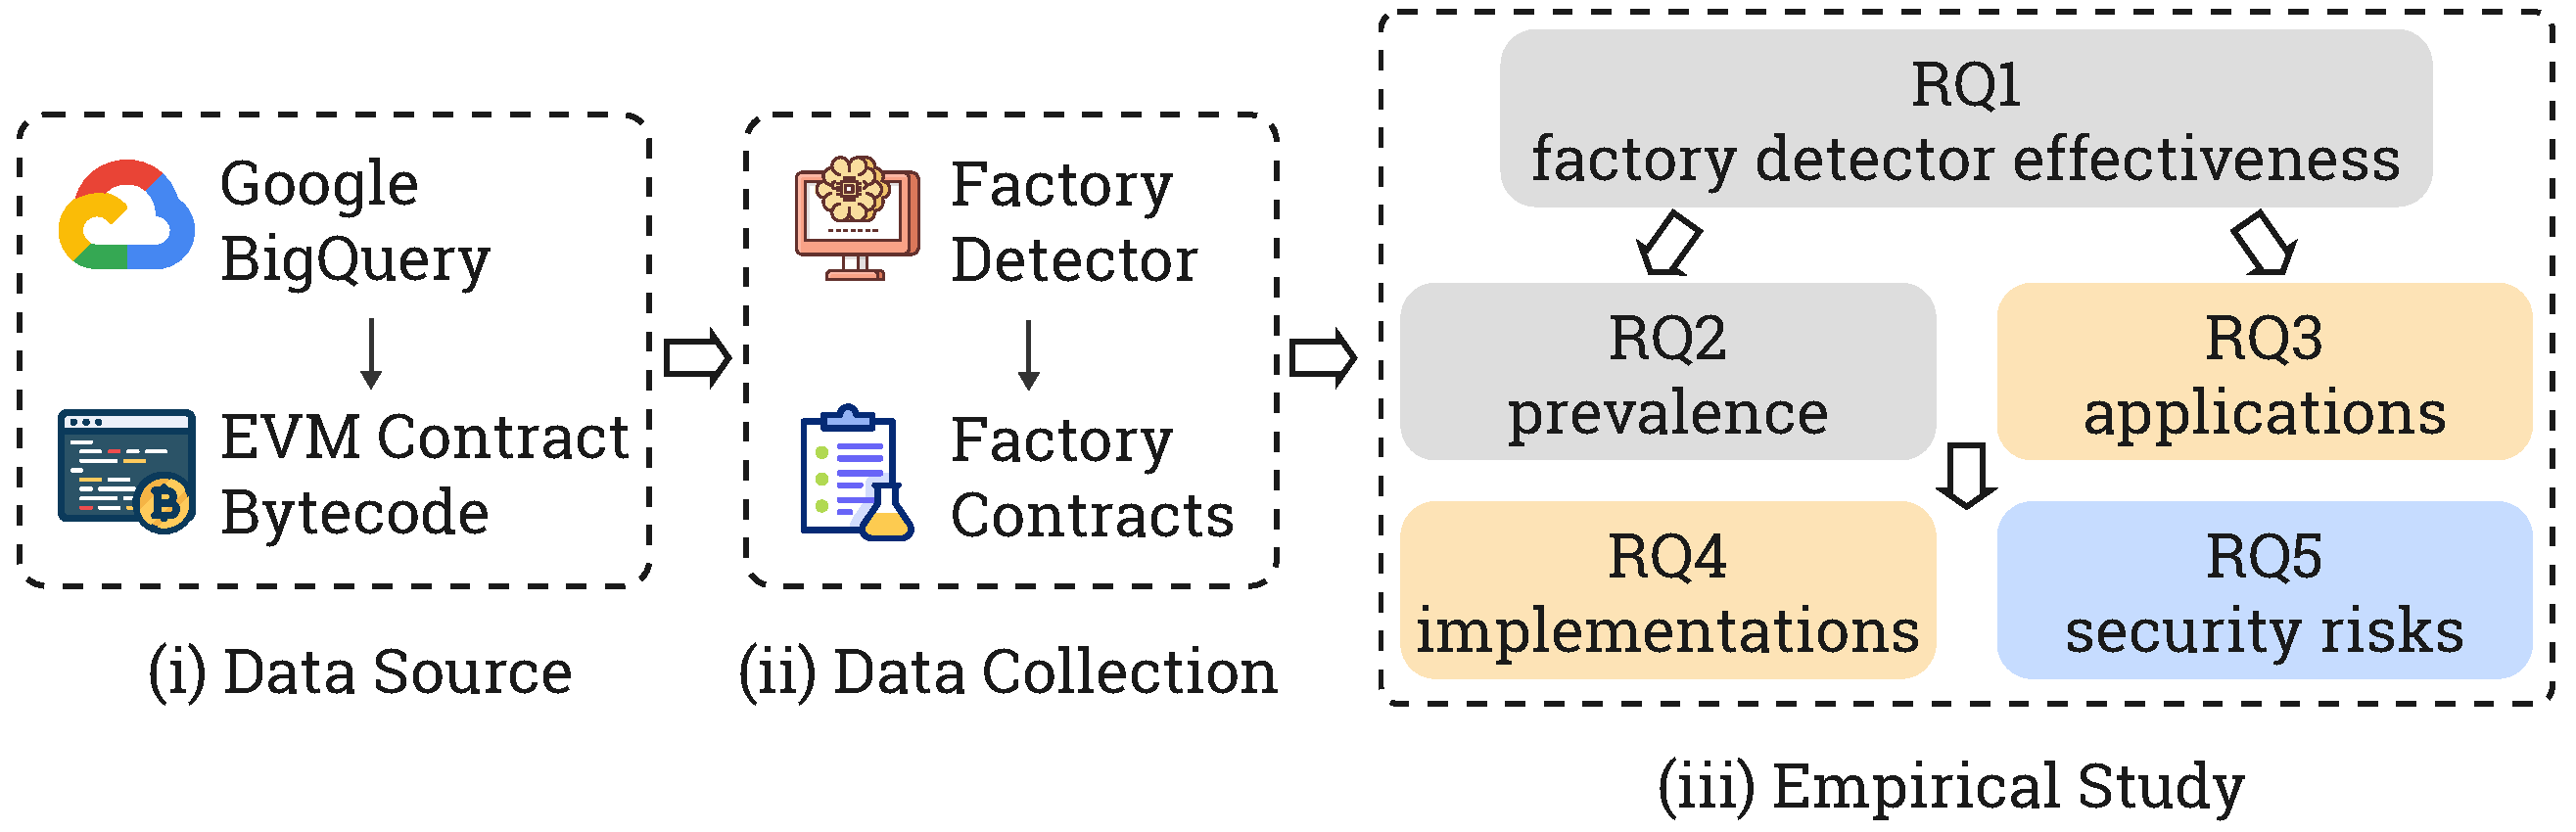
\includegraphics[width=0.9\linewidth]{figure/overview.pdf}
		\caption{Overview of the revised study (RQ1--RQ5), data sources, and analysis flow.}
		\label{fig:overview}
	\end{figure}

	% =====================================================
	\newpage

	\section*{Meta-review from the Editors}

	% Comment 1 — Dataset scope and claims
	\begin{tcolorbox}
		[commentbox,title=Editor/AE -- Comment 1] Qualify ecosystem-wide conclusions given the
		original reliance on verified contracts (small, non-representative subset).
	\end{tcolorbox}

	\noindent
	\textbf{Response.}

	We re-architect the study around bytecode-level analysis and multi-chain coverage (Ethereum and Polygon),
	removing dependence on the small verified subset. We collect and analyze 434,542,165 deployed
	bytecodes and 3,680,947 unique runtimes via BigQuery ({\textbf{RQ2, Methodology, Table dataset}}).
	Claims are now explicitly scoped and supported by bytecode-wide measurements ({\textbf{Bytecode-level, multi-chain, 434M}}).

\vspace{0.25em}
\noindent\textit{Position in revised manuscript:} {\color{red}\textbf{RQ2; Methodology}}
\noindent\textit{Main change:} {\color{blue}\textbf{Multi-chain, bytecode-wide scope with explicit cutoff}}

	% Comment 2 — Detector details and validation
	\begin{tcolorbox}
		[commentbox,title=Editor/AE -- Comment 2] Provide technical details and validation for
		detectors (precision/recall; false positives).
	\end{tcolorbox}

	\noindent
	\textbf{Response.}

	We introduce a bytecode-based Factory Contract Detector with CFG + reachability analysis that
	verifies on-path CREATE/CREATE2 opcodes ({\textbf{RQ1, Algorithm, Fig. execution\_time\_cdf}}). We
	evaluate against a curated ground truth of 2,907 contracts, reporting FPR 0.17\% and FNR 8.39\%
	with execution-time CDF and detailed FN/FP analyses ({\textbf{CFG+reachability; FPR 0.17\%, FNR 8.39\%}}).

\vspace{0.25em}
\noindent\textit{Position in revised manuscript:} {\color{red}\textbf{RQ1}}
\noindent\textit{Main change:} {\color{blue}\textbf{Detector algorithm + precision/recall/timing; FN/FP analyses}}

	% Comment 3 — Clarify FSC vs conventional deployments; distinguish risks
	\begin{tcolorbox}
		[commentbox,title=Editor/AE -- Comment 3] Clarify how FSCs differ from conventional
		deployments and distinguish risks.
	\end{tcolorbox}

	\noindent
	\textbf{Response.}

	Background clarifies EOA vs factory-mediated deployments with a comparative figure, and security
	sections explicitly separate attack vectors vs. security issues and indicate which affect factory-deployed
	vs factory contracts ({\textbf{Background, RQ5}}; {\textbf{Attack vectors vs security issues; factory vs factory-deployed}}).

\vspace{0.25em}
\noindent\textit{Position in revised manuscript:} {\color{red}\textbf{Background; RQ5}}
\noindent\textit{Main change:} {\color{blue}\textbf{Clear separation: targets and risk categories}}

	% Comment 4 — Add concrete case studies and impact
	\begin{tcolorbox}
		[commentbox,title=Editor/AE -- Comment 4] Add concrete case studies and discuss practical
		impact.
	\end{tcolorbox}

	\noindent
	\textbf{Response.}

	Beyond Tornado Cash, we add cases for Address Spoofing via CREATE2, Unhandled Low-Level Contract
	Creation, Unexpected Ownership Transfer (NFT platform), and Unverified Master Contract (NinfaFactory),
	with mitigations ({\textbf{RQ5}}; {\textbf{New cases + actionable mitigations}}).

	\vspace{0.25em}
\noindent\textit{Position in revised manuscript:} {\color{red}\textbf{RQ5}}
\noindent\textit{Main change:} {\color{blue}\textbf{Case studies with concrete mitigations}}

	% Comment 5 — Manual analysis details and Algorithm-1 scope
	\begin{tcolorbox}
		[commentbox,title=Editor/AE -- Comment 5] Provide more manual analysis details and clarify
		Algorithm-1 scope.
	\end{tcolorbox}

	\noindent
	\textbf{Response.}

	We document guidelines, independent reviews, three-round voting, and public artifacts; we scope
	algorithmic descriptions to factory detection pseudocode and security procedures ({\textbf{Threats to Validity, RQ1, RQ5}};
	{\textbf{Guidelines, independent reviews, 3-round voting, artifacts}}).

\vspace{0.25em}
\noindent\textit{Position in revised manuscript:} {\color{red}\textbf{Threats to Validity; RQ1; RQ5}}
\noindent\textit{Main change:} {\color{blue}\textbf{Detailed manual process; clarified algorithm scope; artifacts released}}

	% Comment 6 — Make Section 6.2 (Related Work) more comprehensive
	\begin{tcolorbox}
		[commentbox,title=Editor/AE -- Comment 6] Make Section 6.2 more comprehensive (expand Related
		Work; include broader surveys and non-Ethereum context).
	\end{tcolorbox}

	\noindent
	\textbf{Response.}

	We expand Related Work and discuss external validity across EVM-compatible chains ({\textbf{Related Work, Threats to Validity}};
	{\textbf{Expanded literature; external validity}}). We add discussion of non-Ethereum (other EVM)
	FSCs and surveys where relevant.

\vspace{0.25em}
\noindent\textit{Position in revised manuscript:} {\color{red}\textbf{Related Work; RQ2; Threats to Validity}}
\noindent\textit{Main change:} {\color{blue}\textbf{Broadened literature + cross-chain context}}

	% Comment 7 — Additional editorial suggestions
	\begin{tcolorbox}
		[commentbox,title=Editor/AE -- Comment 7] Address clustering improvements, acknowledge upgradeable-contract
		risks, and discuss generalizability beyond Ethereum.
	\end{tcolorbox}

	\noindent
	\textbf{Response.}

	We redesign clustering with multi-view features and standardized + PCA + KMeans analysis ({\textbf{RQ3}});
	we explicitly surface the Proxy \& Upgrade domain and associated controls ({\textbf{RQ3/RQ4/RQ5}});
	and we extend scope to Ethereum+Polygon with explicit external-validity statements ({\textbf{RQ2; Threats to Validity}}).

	\vspace{0.25em}
\noindent\textit{Position in revised manuscript:} {\color{red}\textbf{RQ3; RQ3/RQ4/RQ5; RQ2; Threats to Validity}}
\noindent\textit{Main change:} {\color{blue}\textbf{Multi-view clustering; upgrade risks acknowledged; multi-chain generalization}}

	% ================== Reviewer 1 =======================
	\newpage
	\section{Comments from Reviewer \#1}

	\begin{tcolorbox}
		[commentbox,title=Reviewer \#1 -- Comment 1] Rewrite Section 6.2 to be more comprehensive and
		add recent surveys; add discussion about non-Ethereum (other EVM) FSCs.
	\end{tcolorbox}

	\noindent
	\textbf{Response.}

	- We expand Related Work with recent literature on deployment, proxies/upgradeability, and smart-contract
	security tooling, improving contextual coverage (Related Work; Expanded coverage).

	- We broaden the empirical scope to EVM-compatible chains by including Polygon in addition to Ethereum
	and discuss external validity/generalizability (RQ2; Threats to Validity; Ethereum+Polygon
	comparisons).

	- If desired, we can further incorporate additional surveys in the next iteration.

\vspace{0.25em}
\noindent\textit{Position in revised manuscript:} {\color{red}\textbf{Related Work; RQ2; Threats to Validity}}
\noindent\textit{Main change:} {\color{blue}\textbf{Expanded literature coverage; multi-chain scope (Ethereum+Polygon)}}

	% ================== Reviewer 2 =======================
	\newpage
	\section{Comments from Reviewer \#2}

	\begin{tcolorbox}
		[commentbox,title=Reviewer \#2 -- Comment 1] Dataset scope is too limited (prior analysis
		relied on the ~<1\% verified-source subset on Ethereum). Please avoid overgeneralizing prevalence
		and security findings; either support them with chain-wide, bytecode-level evidence and an explicit
		cutoff window, or clearly qualify the claims and limitations.
	\end{tcolorbox}

	\noindent
	\textbf{Response.}

	We redesign the study to operate at bytecode level and across Ethereum and Polygon, eliminating reliance
	on verified-only data ({\textbf{RQ2}}). We analyze 434M deployed bytecodes and report prevalence
	from on-chain bytecode evidence ({\textbf{Multi-chain, bytecode-wide prevalence}}), thereby avoiding
	the prior representativeness concern.

\noindent\textit{Position in revised manuscript:} {\color{red}\textbf{RQ2}}
\noindent\textit{Main change:} {\color{blue}\textbf{Multi-chain, bytecode-wide prevalence}}

	\vspace{0.25em}
	For quick reference, Table~\ref{tab:dataset} summarizes the dataset scope and coverage used in
	the revised manuscript.
	\newcolumntype{R}{>{\raggedleft\arraybackslash}X} % Define the "R" column type
\begin{table}[t]
	\centering
	\footnotesize
	\caption{Dataset Overview}
	\label{tab:dataset}
	\begin{tabularx}
		{0.6\linewidth}{@{}lRR@{}} \toprule \textbf{Chain} & \textbf{Total Contract} & \textbf{Unique
		Bytecode} \\ \midrule Ethereum & 73,390,233 & 1,672,444 \\ Polygon & 361,151,932 & 2,008,503
		\\ Total & 434,542,165 & 3,680,947 \\ \bottomrule
	\end{tabularx}
\end{table}


	\begin{tcolorbox}
		[commentbox,title=Reviewer \#2 -- Comment 2] Generalizability of four security detectors;
		support bytecode analysis or acknowledge limitations.
	\end{tcolorbox}

	\noindent
	\textbf{Response.}

	We refocus “detectors” to (i) a rigorously evaluated bytecode-level Factory Contract Detector ( {\textbf{RQ1}}),
	which underpins the empirical study, and (ii) a structured analysis of attack vectors and
	security issues ({\textbf{RQ5}}) supplemented with real cases and mitigations. Rather than reporting
	large-scale auto-detection metrics for each issue, we provide precise technical guidance and
	case-grounded assessments ({\textbf{Detector validated; security framed as vectors+issues}}). We
	also explicitly analyze limitations (e.g., proxy-mediated factories) in RQ1 and Threats to Validity
	({\textbf{Threats to Validity}}).

\noindent\textit{Position in revised manuscript:} {\color{red}\textbf{RQ1; RQ5; Threats to Validity}}
\noindent\textit{Main change:} {\color{blue}\textbf{Detector validated; security framed as vectors+issues}}

	\begin{tcolorbox}
		[commentbox,title=Reviewer \#2 -- Comment 3] Clustering relies on names; incorporate code-based
		features.
	\end{tcolorbox}

	\noindent
	\textbf{Response.}

	We redesign clustering with multi-view features (name tokens, structure/size, mechanism flags,
	access-control/libraries, domain keywords), standardized + PCA (Varimax) + KMeans (k=4) with t-SNE
	visualization ({\textbf{RQ3}}; {\textbf{Multi-view semantics + PCA + KMeans}}).

\noindent\textit{Position in revised manuscript:} {\color{red}\textbf{RQ3}}
\noindent\textit{Main change:} {\color{blue}\textbf{Multi-view semantics + PCA + KMeans}}

	\begin{tcolorbox}
		[commentbox,title=Reviewer \#2 -- Comment 4] Add concrete examples per vulnerability beyond Tornado
		Cash.
	\end{tcolorbox}

	\noindent
	\textbf{Response.}

	We add concrete cases for Address Spoofing via CREATE2, Unhandled Low-Level Contract Creation, Unexpected
	Ownership Transfer (NFT platform), and Unverified Master Contract (NinfaFactory), each with countermeasures
	({\textbf{RQ5}}; {\textbf{Case studies + mitigations}}).

\noindent\textit{Position in revised manuscript:} {\color{red}\textbf{RQ5}}
\noindent\textit{Main change:} {\color{blue}\textbf{Case studies + mitigations}}

	\begin{tcolorbox}
		[commentbox,title=Reviewer \#2 -- Comment 5] Mutable Code detector may have false positives if
		permission checks exist; provide precision/recall or explain handling.
	\end{tcolorbox}

	\noindent
	\textbf{Response.}

	We no longer claim a large-scale automatic detector for Mutable Code. Instead, we treat Mutable Code
	as an attack vector and provide concrete detection/defense guidance and a case study ({\textbf{RQ5}};
	{\textbf{Reachability checks; chain attestation; extcodehash; Tornado case}}). This reframing avoids
	overclaiming and focuses on actionable practice.

\noindent\textit{Position in revised manuscript:} {\color{red}\textbf{RQ5}}
\noindent\textit{Main change:} {\color{blue}\textbf{Reachability checks; chain attestation; extcodehash; Tornado case}}

	\begin{tcolorbox}
		[commentbox,title=Reviewer \#2 -- Typos] Figure reference and USCHunt subject--verb
		agreement.
	\end{tcolorbox}

	\noindent
	\textbf{Response.}

	We correct figure references and fix the subject–verb agreement in Related Work ({\textbf{Related Work}};
	{\textbf{“USCHunt focuses …”}}). We also carefully proofread the manuscript for consistency.

\noindent\textit{Position in revised manuscript:} {\color{red}\textbf{Related Work}}
\noindent\textit{Main change:} {\color{blue}\textbf{Typos fixed; references corrected}}

	% ================== Reviewer 3 =======================
	\newpage
	\section{Comments from Reviewer \#3}

	\begin{tcolorbox}
		[commentbox,title=Reviewer \#3 -- Comment 1] Two initial limitations overlap; clarify
		distinction.
	\end{tcolorbox}

	\noindent
	\textbf{Response.}

	We restructure the Introduction/Abstract to articulate three distinct gaps and align the
	narrative to them (
	{\textbf{Prevalence \& domains; patterns beyond proxies; factory-aware security}}).

	\begin{tcolorbox}
		[commentbox,title=Reviewer \#3 -- Comment 2] Differentiate factory vs. factory-deployed vs. conventional
		EOA deployments, and separate security risks.
	\end{tcolorbox}

	\noindent
	\textbf{Response.}

	Background provides an explicit EOA vs. factory comparison with a deployment figure, and
	security sections indicate which issues impact factory-deployed vs factory contracts; RQ5 headings/captions
	reflect these distinctions ({\textbf{Background, RQ5}}; {\textbf{Clear separation of targets}}).
\noindent\textit{Position in revised manuscript:} {\color{red}\textbf{Background; RQ5}}
\noindent\textit{Main change:} {\color{blue}\textbf{Clear separation of targets}}

	\begin{tcolorbox}
		[commentbox,title=Reviewer \#3 -- Comment 3] Factory detector relies on existing tools;
		unverified contracts via transactions can miss cases.
	\end{tcolorbox}

	\noindent
	\textbf{Response.}

	We design and implement a bytecode-based Factory Contract Detector independent of source code, and
	validate it on a curated ground truth with precision/recall and timing metrics ({\textbf{RQ1}}; {\textbf{Detector validated}}).
	We analyze the principal limitation (proxy-mediated factories) and scope it in Threats to Validity
	({\textbf{Threats to Validity}}).

	\begin{tcolorbox}
		[commentbox,title=Reviewer \#3 -- Comment 4] 1,180 security issues claim lacks detector design
		details and validation.
	\end{tcolorbox}

	\noindent
	\textbf{Response.}

	We no longer claim a fixed issue count. Instead, we provide an attack-vector–driven analysis
	with real-world cases and mitigations ({\textbf{RQ5}}), while rigorously validating the foundational
factory detector ({\textbf{RQ1}}).
\noindent\textit{Position in revised manuscript:} {\color{red}\textbf{RQ5; RQ1}}
\noindent\textit{Main change:} {\color{blue}\textbf{Vector-driven security; validated detector}}

	\begin{tcolorbox}
		[commentbox,title=Reviewer \#3 -- Comment 5] Exclusively Ethereum; generalizability to other
		EVM chains is limited.
	\end{tcolorbox}

	\noindent
	\textbf{Response.}

	We extend to Polygon and discuss external validity and future extensions ( {\textbf{RQ2; Threats to Validity}}).
\noindent\textit{Position in revised manuscript:} {\color{red}\textbf{RQ2; Threats to Validity}}
\noindent\textit{Main change:} {\color{blue}\textbf{Multi-chain study; external validity}}

	\begin{tcolorbox}
		[commentbox,title=Reviewer \#3 -- Comment 6] Quantify economic impact; add real-world
		exploits beyond Tornado Cash.
	\end{tcolorbox}

	\noindent
	\textbf{Response.}

	We add case-grounded analyses on Address Spoofing, Unhandled Low-Level Creation, Unexpected
	Ownership Transfer, and Unverified Master Contract with practical consequences and mitigations (
	{\textbf{RQ5}}). Where precise loss amounts require on-chain forensics, we scope this as future
	work and provide concrete operational guidance now ({\textbf{Practice-first; quantification planned}}).
\noindent\textit{Position in revised manuscript:} {\color{red}\textbf{RQ5}}
\noindent\textit{Main change:} {\color{blue}\textbf{Cases with mitigations; quantification planned}}

	% ================== Reviewer 4 =======================
	\newpage
	\section{Comments from Reviewer \#4}

	\begin{tcolorbox}
		[commentbox,title=Reviewer \#4 -- Comment 1] Manual analysis depends on experts; please
		include auditors' background, time commitment, and conflict resolution.
	\end{tcolorbox}

	\noindent
	\textbf{Response.}

	We document predefined auditing guidelines, independent reviews, three-round voting, and expert
	discussions, and we release public artifacts ({\textbf{Threats to Validity}}; {\textbf{Guidelines + 3-round expert reviews}}).
	Due to space and anonymization constraints, we summarize process rather than full biographies; upon
	request, we can provide de-identified expertise profiles and time accounting in the artifact
documentation.
\noindent\textit{Position in revised manuscript:} {\color{red}\textbf{Threats to Validity}}
\noindent\textit{Main change:} {\color{blue}\textbf{Guidelines + 3-round expert reviews; artifacts released}}

	\begin{tcolorbox}
		[commentbox,title=Reviewer \#4 -- Comment 2] No ground-truth to estimate tool effectiveness;
		did you validate all reported issues? detectors missing/misreporting?
	\end{tcolorbox}

	\noindent
	\textbf{Response.}

	We introduce a curated ground-truth for factory detection and thoroughly evaluate it ({\textbf{RQ1}};
	{\textbf{Precision/recall/timing; FN/FP analyses}}). For security issues, we pivot from mass counting
		to case-backed analyses and mitigations, avoiding overclaims ({\textbf{RQ5}}).
		\noindent\textit{Position in revised manuscript:} {\color{red}\textbf{RQ1; RQ5}}
		\noindent\textit{Main change:} {\color{blue}\textbf{Precision/recall/timing + FN/FP analyses; case-backed security}}

	\begin{tcolorbox}
		[commentbox,title=Reviewer \#4 -- Comment 3] Lack of severity evaluation of discovered issues.
	\end{tcolorbox}

	\noindent
	\textbf{Response.}

	For each issue/vector we discuss practical impact and operational risks with prioritized
	mitigations ({\textbf{RQ5}}; {\textbf{Return-value validation; chain attestation}}). We plan to
		add broader economic quantification in future work as on-chain datasets for losses mature.
		\noindent\textit{Position in revised manuscript:} {\color{red}\textbf{RQ5}}
		\noindent\textit{Main change:} {\color{blue}\textbf{Return-value validation; deployment-chain attestation}}

	\begin{tcolorbox}
		[commentbox,title=Reviewer \#4 -- Comment 4] Technical novelty: many patterns are known; contributions
		appear cataloging and rule-based.
	\end{tcolorbox}

	\noindent
	\textbf{Response.}

	We deliver a novel, validated bytecode-level detection infrastructure at ecosystem scale, multi-chain
	measurements, and a structured, factory-aware security analysis with concrete mitigations (
	{\textbf{Beyond cataloging; actionable security}}).

	\begin{tcolorbox}
		[commentbox,title=Reviewer \#4 -- Comment 5] Presentation: typos; Algorithm-1 unclear and only
		for part of the analysis.
	\end{tcolorbox}

	\noindent
	\textbf{Response.}

	We add full pseudocode for the Factory Contract Detector (RQ1) and clarify scope for other
analyses with detailed procedures, examples, and figures. We correct typos (including USCHunt
“focuses”) and audited cross-references.
\noindent\textit{Position in revised manuscript:} {\color{red}\textbf{RQ1}}
\noindent\textit{Main change:} {\color{blue}\textbf{Algorithm pseudocode added; scope clarified; typos fixed}}

	\vspace{1em}
	\noindent
	We appreciate the reviewers’ insights and believe the revised manuscript addresses the major
	concerns through bytecode-level, multi-chain measurement; validated detection infrastructure; richer
	clustering and security analyses; and clearer methodology and threats-to-validity discussions. All
	artifacts are released for reproducibility.
\end{document}
